%!TEX root = ../thesis.tex
% створюємо розділ
\chapter{Генеративні моделі у задачах сегментації супутникових знімків}
\label{chap:gans}

У другому розділі ми розглянемо генеративні моделі, які можуть
бути застосовані для генерації штучних супутникових знімків.
Особлива увага буде приділена генеративно-змагальним нейронним
мережам. Також піде мова про вирішення задачі image-to-image translation
за допомогою GAN, а саме про архітектуру Pix2Pix та її вдосконалені версії.
Та нарешті буде описано механізм застосування генеративно-змагальних мереж
для аугментації навчальних вибірок, що має за мету вирішити проблеми, які
були описані у попередньому розділі.

\section{Різновиди генеративних моделей}

Для того, щоб наблизитись до розв'язку проблеми генерації
штучних зображень,
розглянемо наступну задачу:
нехай існує набір даних $(x_1, x_2, \dots) \in X$,
які мають невідомий розподіл $\pi$.
Ми намагаємось знайти його оцінку
$$p^* \in \arg \min\limits_{p} \mathcal{D}(\pi || p),$$
де $\mathcal{D}$ - деяка
міра близькості розподілів, яка задовольняє умови
\begin{equation*}
    \begin{cases}
        \mathcal{D}(\pi || p) \geq 0, & \pi \neq p \\
        \mathcal{D}(\pi || p) = 0,    & \pi = p
    \end{cases}
\end{equation*}

Наприклад дивергенція Йонсена-Шеннона:
\begin{equation} \label{eq:jsd}
    JSD(\pi || p) = \frac{1}{2} \int\limits_{\mathbb{R}}
    \left[
        \pi(x) \ln \frac{2\pi(x)}{p(x) + \pi(x)} +
        p(x) \ln \frac{2p(x)}{p(x) + \pi(x)}
        \right] dx
\end{equation}

Якщо ми зможемо знайти дану оцінку розподілу для
реальних супутникових знімків, то ми зможемо
генерувати випадкові величини з даного розподілу, які
і будуть являти собою штучні знімки. Звичайно, що
пошук по усім можливим розподілам є дуже складною задачею,
тому ми зосередимось на параметричних моделях, тобто:
$$p(x | \theta) \in \arg \min\limits_{\theta} \mathcal{D}(\pi || p_\theta),$$

Існує багато методів розв'язку подібних задач, які можна поділити
на декілька великих груп \cite{goodfellow2016nips},
що зображено на рисунку \ref{fig:gen_models}.

\begin{figure}[!ht]
    \centering
    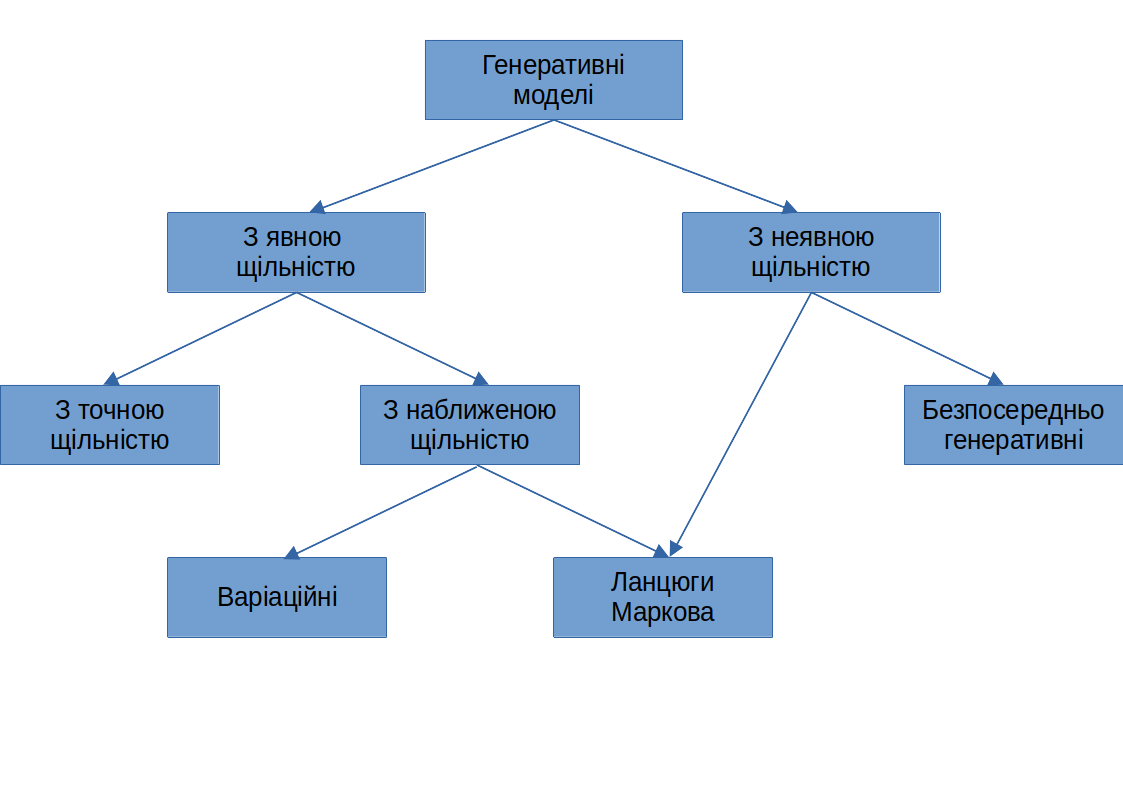
\includegraphics[width=0.9 \textwidth]{gen_models.png}
    \caption{Таксономія генеративних моделей}
    \label{fig:gen_models}
\end{figure}

Моделі з явною щільністю дозволяють обраховувати значення щільності.
Максимізація правдоподібності для даних моделей є простою,
бо являє собою просту підстановку щільності, що описує модель,
у вираз для правдоподібності. Найскладніше для даної групи
підібрати таку модель, яка зможе описувати усю складність реальних даних
і при цьому дозволить обраховувати щільність розподілу.
Тому виділяють дві стратегії:
\begin{enumerate}
    \item моделі, які гарантують можливість точного обрахунку (tractability);
    \item моделі, які ґрунтуються на обрахунку наближених значень.
\end{enumerate}

Моделі, які гарантують можливість точного обрахунку щільності, такі як
FVBN (fully visible belief networks), нормалізуючи потоки, мають перевагу у тому,
що дозволяють проводити оптимізацію безпосередньо функції
правдоподібності, проте це вимагає від них жорстких обмежень.
До того ж більшість подібних моделей виконують обрахунки послідовно,
тобто для генерації необхідно виконати декілька послідовних кроків, які
не можуть бути розпаралелині, що значно збільшує час необхідний для
генерації.

Для уникнення проблем, пов'язаних з жорсткими обмеженнями на
модель, які необхідні для точно обрахунку щільності, використовуються
моделі, які дозволяють отримувати наближені значення щільності.
Вони у свою чергу поділяються на дві групи: з детерміністичною
апроксимацією, здебільшого це автоенкодери, та зі стохастичною,
як наприклад ланцюги Маркова, машини Больцмана.

Звичайно, що і у даних підходів є суттєві недоліки.
Варіаційні автоенкодери використовують у своїй роботі
нижню границю (ELBO), яка при виборі "слабкого" апостеріорного
або ж апріорного може значно відрізнятися від справжньої
правдоподібності, що призведе до того, що розподіл генератора
та реальний розподіл будуть значно відрізнятись. На практиці
варіаційні моделі все ж здатні гарно апроксимувати правдоподібність,
проте якість згенерованих зображень є низькою. Якщо ж казати про
недоліки методів побудованих на основі ланцюгів Маркова, то
слід зазначити їх низьку швидкодію, що обумовлена як необхідністю
виконувати операції покроково, так і тим, що збіжність
дужу повільна та не має жодного методу, який би міг вказати
чи вже наявна збіжність чи потребується продовжити оптимізацію.

Концептуально іншим підходом є застосування моделей, які
не оперують щільністю або її наближеннями як такими, а
навчаються лише ґрунтуючись на тих прикладах, які надає
генератор. Тобто використовують не сам розподіл як такий, а
певні спостереження з нього. Деякі з цих моделей знову ж таки
використовують ланцюги Маркова для генерування прикладів,
здебільшого це генеративні стохастичні мережі. Але вони мають
притаманні усім ланцюгам Маркова недоліки, які були описані вище.
І на сам кінець існують моделі, які здатні безпосередньо
генерувати зображення за один крок. Найбільш відомими й поширеними з них
є генеративно-змагальні мережі, які ми розглянемо більш детально.

\section{Генеративно-змагальні мережі}

Ідея оригінальної GAN  \cite{goodfellow2014generative}
полягає у тому, що ми маємо дві сутності:
генератор --- диференційовну функцію $G: Q \times \Theta_G \rightarrow X$, яка
на основі елементу з множини $Q$ (так званого латентного простору)
та параметрів $\theta_g \in \Theta_G$
генерує елемент з множин $X$; та дискримінатор
--- диференційовну функцію $D: X \times \Theta_D \rightarrow \{0, 1\}$, яка
намагається на визначити чи є елемент штучно згенерованим, чи
належить розподілу навчальних даних. Для пошуку функції
генератора та дискримінатора застосовується міні-максний функціонал якості:
\begin{equation} \label{eq:gan_criterion}
    \min\limits_{G}\max\limits_{D} \left[
        \E_{x \sim \pi} \ln D(x) +
        \E_{q \sim p_{Q}} \ln (1 - D(G(q))) \right],
\end{equation}

Тобто відбувається змагання між генератором, який прагне генерувати найбільш
схожі на реальні зображення, щоб ввести в оману дискримінатор,
який навпаки прагне якомога краще відрізняти штучно згенеровані та
реальні приклади.

Але для того, щоб знайти відповідні оптимальні значення
параметрів дискримінатора та генератора необхідний алгоритм навчання,
який з кожним кроком буде все ближче і ближче наближати розподіл
генератора до реального, аж поки дискримінатор не втратить будь-яку можливість
відрізняти реальні та штучно згенеровані зображення. Дану ідею
зображено на рисунку \ref{fig:gan}.

\begin{figure}[h]
    \centering
    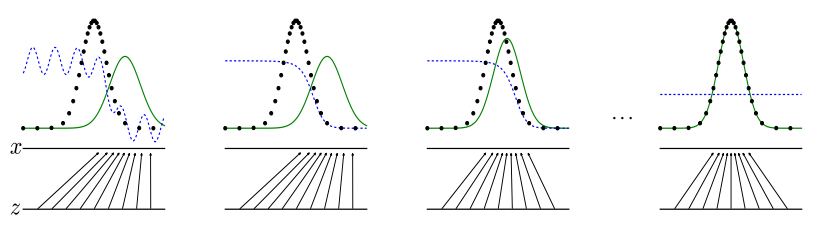
\includegraphics[width=0.75 \textwidth]{gan_distribution.png}
    \caption{Ілюстрація ідеї GAN \cite{goodfellow2014generative}.
        Зеленим позначено розподіл генератора,
        синім --- дискримінатора,
        чорними точками --- реальних даних}
    \label{fig:gan}
\end{figure}

Як це притаманно
штучним нейронним мережам, алгоритм оптимізації ґрунтується на
обрахунку і використанні градієнтів цільової функції помилки
від параметрів. Але, через те, що наша модель не є класичною
нейромережею, необхідний окремий підхід до навчання GAN.

\begin{algorithm}[Алгоритм навчання GAN]

    Параметри: $k$ - кількість ітерацій навчання дискримінатора за 1 епоху,
    $N$ - кількість епох навчання, $m$ - розмірність батчу.

    Вхідні дані: навчальна вибірка $X$ з розподілом $\pi$.

    \begin{enumerate}
        \item Доки кількість епох навчання не досягла $N$
              \begin{enumerate}
                  \item Повторювати $k$ разів
                        \begin{enumerate}[leftmargin=3.25cm]
                            \item Згенерувати $\{z_1, \dots, z_m\}$
                            \item Обрати $\{x_1, \dots, x_m\} \sim \pi(x)$
                            \item Оновити параметри дискримінатора використовуючи градієнт
                                  \begin{equation*}
                                      \nabla_{\theta_D} \left( \frac{1}{m}\sum\limits_{i=1}^m \left[
                                              \ln D(x_i) + \ln (1 - D(G(z_i))) \right] \right)
                                  \end{equation*}
                        \end{enumerate}
                  \item Згенерувати нові $\{z'_1, \dots, z'_m\}$\;
                  \item Оновити параметри генератора використовуючи градієнт
                        \begin{equation*}
                            \nabla_{\theta_G} \left( \frac{1}{m}\sum\limits_{i=1}^m
                            \ln (1 - D(G(z'_i))) \right)
                        \end{equation*}
              \end{enumerate}
    \end{enumerate}
\end{algorithm}

У якості оптимізатора, який використовує вже обраховані градієнти
можна застосовувати довільний алгоритм, у більшості випадків це або
звичайний градієнтний спуск,
або більш досконалі методи, як наприклад
Adam \cite{kingma2014adam}.

Окремим питанням, яке заслуговує на увагу, є питання про те,
а чи дійсно у результаті розв'язку цієї задачі ми отримаємо
генератор, розподіл якого дорівнює розподілу реальних даних.
Для того, щоб переконатися у цьому доведемо дві важливі теореми.

\begin{theorem}[Гудфелоу \cite{goodfellow2014generative}]
    Для фіксованого генератора $G$ з розподілом $p_G(x)$
    оптимальним дискримінатором $D^*(x)$ є:
    \begin{equation*}
        D^{*}(x) = \frac{\pi(x)}{\pi(x) + p_G(x)}.
    \end{equation*}
\end{theorem}
\begin{proof}
    Запишемо цільову функцію:
    \begin{equation*}
        \min\limits_{G}\max\limits_{D} \left[
            \E_{x \sim \pi} \ln D(x) +
            \E_{q \sim p_{Q}} \ln (1 - D(G(q))) \right]
    \end{equation*}
    Генератор, за припущенням є фіксованим, тож ми можемо перейти
    від математичного сподівання по латентному просторі до математичного сподівання
    розподілу генератора $p_G(x)$.
    \begin{equation*}
        \min\limits_{G}\max\limits_{D} \left[
            \E_{x \sim \pi} \ln D(x) +
            \E_{x \sim G(x)} \ln (1 - D(x)) \right]
    \end{equation*}
    Наступним кроком розпишемо математичні сподівання та
    властивостями визначених інтегралів:
    \begin{equation*}
        \min\limits_{G} \int\limits_X \max\limits_{D}
        \left( \pi(x) \ln D(x) +
        p_G(x) \ln (1 - D(x)) \right) dx
    \end{equation*}
    Розглянемо умову екстремум для виразу під
    знаком максимуму і отримаємо:
    \begin{gather*}
        \frac{\partial}{\partial D(x)}
        \left( \pi(x) \ln D(x) +
        p_G(x) \ln (1 - D(x)) \right) = \\
        = \frac{\pi(x)}{D(x)} - \frac{p_G(x)}{1 - D(x)} = 0
    \end{gather*}
    І виразивши $D(x)$ остаточно отримаємо:
    \begin{equation*}
        D^{*}(x) = \frac{\pi(x)}{\pi(x) + p_G(x)}
    \end{equation*}
\end{proof}

\begin{theorem}[Гудфелоу \cite{goodfellow2014generative}]
    Глобальний мінімум критерію \eqref{eq:gan_criterion} досягається
    тобі і тільки тоді, коли розподіли генератора $p_G$ та реальних даних
    однакові. При цьому значення критерію дорівнює $-\ln 4$.
\end{theorem}
\begin{proof}
    Підставимо оптимальний дискримінатор у критерій~\eqref{eq:gan_criterion}.
    \begin{equation*}
        \min\limits_{G} \left[
            \E_{x \sim \pi} \ln \frac{\pi(x)}{\pi(x) + p_G(x)} +
            \E_{q \sim p_G} \ln \frac{\pi_G(x)}{\pi(x) + p_G(x)}
            \right]
    \end{equation*}
    Тепер помножимо і поділимо кожен дріб на 2 та використаємо властивість
    логарифмів та математичного сподівання від константи.
    \begin{equation*}
        \min\limits_{G} \left[
            \E_{x \sim \pi} \ln \frac{2 \pi(x)}{\pi(x) + p_G(x)} +
            \E_{q \sim p_G} \ln \frac{2 \pi_G(x)}{\pi(x) + p_G(x)}
            \right] - \ln 4
    \end{equation*}
    Вираз у дужках є нічим іншим як дивергенцією Йонсена-Шеннона \eqref{eq:jsd}.
    Вона приймає мінімальне значення $0$ тоді і тільки тоді, коли
    розподіли дорівнюють один одному. І, відповідно, значення критерію
    у випадку рівності $0$ мінімуму буде дорівнювати $-\ln 4$.
\end{proof}

Проте наявний алгоритм навчання майже завжди не використовується
на практиці, що пов'язано з тим, що градієнти параметрів генератора
згасають \cite{arjovsky2017towards, goodfellow2014generative}.
Це є наслідком самої будови функції помилки, тому її заміняють
на наступний аналог:

\begin{equation} \label{eq:gan_generator_loss}
    - \ln D(G(z))
\end{equation}

Притаманні процесу навчання генеративно-змагальних мереж і інші проблеми,
як наприклад нестабільність навчання, яка полягає у тому, що
у деяких випадках алгоритм не може знайти оптимальні
дискримінатор та генератор. Деякі причини цього детально
описані у роботі \cite{arjovsky2017towards}, серед них нестабільність
градієнтів функції помилки у вигляді \eqref{eq:gan_generator_loss}.
Іншою можливою причиною може бути те, що як зображено на рис. \ref{fig:gan},
з кожною ітерацією генератор покращується, що робить зворотній
зв'язок від дискримінатора все менш правильним, і на сам кінець зовсім випадковим.
Тобто генератор починає вчитися на небажаному зворотному зв'язку від дискримінатора.

Одним зі шляхів подолання даних проблем є додавання шуму до
входу дискримінатора, застосування спектральних нормалізацій \cite{miyato2018spectral} або
ж регуляризацій \cite{roth2017stabilizing}.

Іншою істотною проблемою є так званий mode collapse.
Вона полягає у тому, що вихідні зображення дуже мало
відрізняються один від одного та модель не в змозі генерувати
різноманітні приклади. Це відбувається через те, що генератор
завжди намагається ввести в оману дискримінатор, і для цього
генерує зображення, які з найбільшою ймовірністю будуть розпізнанні
дискримінатором як справжні. Але якщо виявилось так, що
дискримінатор потрапив у локальний максимум, з якого не може вибратись,
то генератор надмірно пристосовується саме до цього дискримінатора, через
що і генерує невелике розмаїття зображень.

Зміна дискримінатора та критерію оптимізації спроможні подолати
дану проблему. Одним з таких підходів є Wasserstein GAN \cite{arjovsky2017wasserstein}.
Який змінює дискримінатор, який приймає обмежені значення на критика,
виходи якого можуть бути довільні. До того ж сама функція помилки
була змінена на таку, що відображає відстань між розподілами.
Серед усього іншого, даний підхід спроможний допомогти і
у випадку нестабільного навчання.

Попри усі згадані недоліки, якість зображень та швидкодія генерації
штучних прикладів для генеративно-змагальних мереж є
високою, що і робить GAN визнаним спільнотою лідером у задачах
генерації штучних зображень.

Підсумовуючи, генеративно-змагальні мережі мають наступні
переваги над іншими моделями:
\begin{enumerate}
    \item Можливість паралельної генерації,
          що забезпечує швидкість роботи навченої моделі.
    \item На генератора накладається мало обмежень, що дає можливість
          вибору широко класу архітектур.
          Це є перевагою порівняно з машинами Больцмана,
          які допускають лише певні класи  ймовірнісних розподілів,
          а також щодо потоків, що нормалізують, які вимагають, щоб генератор
          мав зворотнє відображення, а розмірність латентного простіру
          дорівнювала розмірності даних.
    \item Не використовуються ланцюги Маркова з усіма їх
          недоліками, як у машинах Больцмана та генеративних стохастичних мережах.
    \item Генеративна мережа, оптимізація якої була збіжною, точно наближає
          розподіл реальних даних, а не використовує нижні чи верхні
          оцінки, як це у випадку з автоенкодерами.
    \item Якість зображень, які генеруються за допомогою GAN,
          здебільшого вища за інші моделі.
\end{enumerate}

Саме ці моменти і обумовлюють вибір саме генеративно-змагальних
мереж для генерації штучних супутникових знімків, і, як наслідок,
аугментації навчальних вибірок.

\section{GAN у задачах image-to-image translation}

Для того, щоб мати вплив на згенеровані класичними
генеративно-змагальними мережами зображення, ми маємо
досліджувати структуру латентного простору, і навіть якщо нам
це, використовуючи певні методи, вдасться, у нас все ще не буде
повного контролю за кожним пікселем зображення, бо
розмірність латентного простору майже завжди менша за
розмірність зображення. Таким чином точно контролювати розподіл класів у
згенерованих зображеннях не є можливим.

Наша ж задача полягає саме у тому, щоб генерувати штучні супутникові
знімки і при цьому мати знання про клас кожного зі згенерованих
пікселів. Саме тому нам потрібно звернути увагу на ті методи, які дозволять
контролювати кожний з вихідних пікселів.

Однією з задач, яка влаштовує наші вимоги є задача image-to-image translation,
яка полягає у тому, що ми повинні перетворити зображення з одного домену у інший, при цьому кількість
каналів вхідного та вихідного зображення не повинна бути однаковою.
Таким чином подавши маски, на яких будуть зазначені класи кожного з пікселів,
ми зможемо генерувати штучні супутникові знімки, з потрібним нам
відношенням класів.

Наївні підходи до розв'язку даної задачі, які полягають у навчанні
звичайної згорткової нейронної мережі з мінімізацією евклідової відстані,
призведуть до того, що значення пікселів кожного з класів будуть
усереднені. І, відповідно, ми отримаємо згенеровані зображення
дуже низької якості. Тож слід звернути увагу на GAN, які дозволять
задати кінцеву ціль у вигляді <<зробити згенеровані
зображення такими, що складно відрізнити від справжніх>>.

Існує цілий клас генеративно-змагальних мереж, які дозволяють вирішувати дану
задачу. Це так звані умовні (conditional) GAN. Однією з провідних
архітектур, саме у задачі image-to-image translation, є Pix2Pix~\cite{pix2pix}.

Першим істотної відмінністю архітектури Pix2Pix від
класичних GAN є функція помилки, а саме: для вхідного зображення
$x$ та бажаного вихідного зображення $y$ вона виглядає
наступним чином:

\begin{equation} \label{eq:pix2pix_loss}
    \E_{x, y} \log D(x,y) +
    \E_{x} \log (1 - D(x, G(x))) +
    \lambda_{L_1} \E_{y, x} ||y - G(x)||_1
\end{equation}

Тобто функція помилки являє собою поєднання класичної помилки
для генеративно-змагальних мереж, з тією зміною, що дискримінатор приймає
два аргументи, і $L_1$ помилки. Перша частина як і у всіх інших
GAN відповідає за те, щоб згенеровані зображення виглядали подібними
до реальних, а друга частина, намагається досягти
попіксельної однаковості між справжніми та штучними знімками.
$L_1$ помилка була обрана авторами \cite{pix2pix}, бо їх досліди
показали, що використання $L_2$ помилки призводить до більшого
рівня розмитості на вихідних зображеннях.

Наступною відмінністю архітектури Pix2Pix є використання так званого
PatchGAN у якості дискримінатора. Він аналізує справжність не усього
зображення, а лише окремих його частин, і потім усереднює отримані результати.
Це дозволяє ефективно моделювати вихідне зображення як
випадкове поле Маркова, при умові, що припускається
незалежність між пікселями, які потрапили у різні частини.
Це можна розуміти \cite{pix2pix} як текстурну помилку або помилку стилю.

При чому слід звернути увагу на те, що дискримінатор приймає
вхідне та вихідне зображення, тобто має змогу
порівняти а чи відповідає згенероване зображення тому
входу, який був поданий на генератор.

Генератор повинен генерувати вихідне зображення такого ж
розміру який мало вхідне, тож цілком закономірно очікувати,
що архітектура генератора повинна бути більш-менш симетричною.
Однією з таких, добре відомих архітектур, є вже розглянута
нами архітектура UNet. Вона добре зарекомендувала себе у
задачах семантичної сегментації, які дещо схожі на задачу image-to-image translation.
До того ж використання особливості UNet дозволяють враховувати як
високорівневі, так і низькорівневі ознаки. Саме ґрунтуючись на цих
принципах, автори \cite{pix2pix} і запропонували використати
варіацію архітектури UNet у якості генератора.

Таким чином повністю архітектуру Pix2Pix можливо подати за допомогою наступної
діаграми (рис. \ref{fig:pix2pix}).

\begin{figure}[!ht]
    \centering
    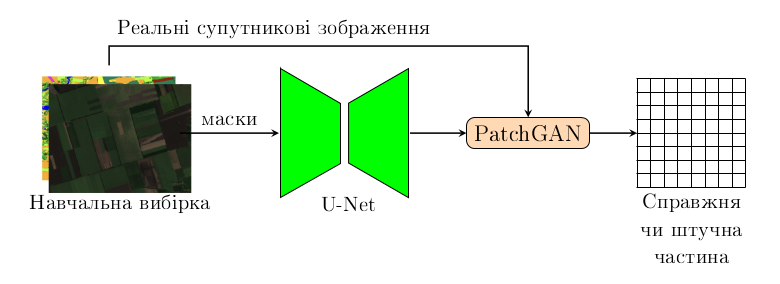
\includegraphics[scale=0.5]{pix2pix.png}
    \caption{Архітектура Pix2Pix у застосуванні до супутникових знімків}
    \label{fig:pix2pix}
\end{figure}

Проте результати роботи запропонованої архітектури інколи
бажають покращення, особливо коли мова йде про генерацію
деталізованих зображень або зображень великої розмірності.
Проте Pix2Pix був і залишається потужною базою, на якій
ґрунтуються більш досконалі методи. Одним з таких є архітектура
Pix2PixHD \cite{pix2pixHD}.

У Pix2PixHD було запропоновано багато вдосконалень класичного
Pix2Pix, серед яких були значні зміни генератора, проте
ці зміни пов'язані з бажанням генерувати саме зображення
більшого розміру. До того ж даний генератор вимагає
більших обчислювальних ресурсів. Ми ж зосередимось на
тих нововведеннях, які мають на меті покращення, у тому числі,
якості зображень.

Першим нововведенням є застосування декількох дискримінаторів.
Кожний з цих дискримінаторів має архітектуру PatchGAN та застосовується
при різних розмірах зображень. Для отримання піраміди зображень
з різними розмірами використовується операція pooling, яка зменшує
у 2 рази. Таким чином різні дискримінатори мають різні рецептивні
поля, що дозволяє їм разом враховувати різні рівні освідомлення
зображення та змінювати генератор так, щоб він генерував
глобально узгоджені результати. Результуюча оцінка ж такого
складеного дискримінатора являє собою суму оцінок кожної
зі складових частин.

Наступні покращення пов'язані з використанням додаткових
функцій помилок. Перша з них являє собою так звану помилку
відповідності ознак. Даний критерій дозволяє стабілізувати
процес навчання за рахунок того, що ми спонукаємо генератор
продукувати зображення, статистики яких будуть наближеними
до реальних при різних масштабах. А саме: дана функція помилки
обраховується за допомогою результатів внутрішніх шарів усіх
дискримінаторів, і призводить до того, що внутрішні представлення
дискримінаторів для штучних та справжніх зображень повинні бути
наближені один до одного. Позначивши як $D_l$ дискримінатор $l$ та, відповідно,
$D_l^{(i)}$ -- вихід $i$-го шару $l$-го дискримінатора, дану похибку можна
подати у вигляді:

\begin{equation} \label{eq:fm_loss}
    L_{FM}(G, D_k) = \E_{x, y} \sum\limits_{i=1}^T
    \frac{1}{N_i} || D^i_k(x, y) - D^i_k(x, G(x)) ||_1,
\end{equation}
де $T$ -- загальна кількість шарів дискримінатора, $N_i$ -- кількість
елементів на шарі $i$. Для обрахунку ж внеску у загальну помилку,
значення сумуються за усіма дискримінаторами та множаться
на константу $\lambda_{FM}$.

Друга функція помилки, яка була представлена і застосована у
\cite{pix2pixHD}, є помилкою, яка основана на тому, щоб
порівнювати внутрішні представлення не тільки дискримінатора,
який постійно перебуває у процесі навчання, а і іншою згорткової
навченої мережі. А саме, її можна представити наступним чином:

\begin{equation} \label{eq:perceptual_loss}
    L_{VGG} = \sum\limits_{i=1}^T
    \frac{1}{N_i} || F^i_k(y) - F^i_k(G(x)) ||_1,
\end{equation}
де $F^i_k$ -- $i$-ий шар навченої згорткової нейромережі,
у більшості випадків використовується VGG,
$T$ -- загальна кількість шарів цієї мережі,
$N_i$ -- кількість елементів на шарі $i$.

Ідея її застосування даної помилки ґрунтується на тому, що
високорівневі внутрішні ознаки навченої глибокої згорткової
нейромережі для згенерованих та справжніх зображень не повинні
сильно відрізнятися.

Таким чином використавши ці покращення ми зможемо
отримати більш якісні згенеровані зображення, проте питання а
чи допоможуть нам аугментовані вибірки отримані таким видозміненим
генератором досягти більшої точності семантичної сегментації залишається
відкритим і буде досліджено у наступних розділах даної роботи.

\section{Перспективи застосування GAN для генерації штучних супутникових знімків}

Маючи ефективні нейромережеві архітектури для розв'язку задачі
image-to-image translation ми в змозі перейти до
генерації аугментованих навчальних вибірок. Ідея даного процесу
полягає у тому, що ми на основі штучних масок з мітками класів,
будемо генерувати штучні супутникові знімки. Ці штучні маски у
свою чергу будуть такими, що допоможуть збільшити сумарну кількість
пікселів для потрібних міноритарних класів і таким чином збалансувати
навчальну вибірку. Це у кінцевому результаті очікувано має дати
кращі показники якості сегментації, при застосуванні доповнених
навчальних матеріалів, отриманих за цією процедурою. Схематично даний процес
можна зобразити як на рисунку \ref{fig:pipline}.

Архітектура Pix2Pix і її варіації є потужним підґрунтям для
реалізація даного процесу, бо дозволяє генерувати якісні зображення,
і при цьому надає нам змогу контролювати клас кожного пікселя,
без чого неможливо створення штучних вибірок для задачі семантичної сегментації.
Окремої уваги заслуговує той факт, що хоч ми і розглядаємо
методи покращення згенерованих зображень, все ж таки
вирішальним для нас є саме покращення якості семантичної сегментації,
особливо щодо міноритарних класів. Тому гонитва за тим, щоб
штучно згенеровані за допомогою генеративно-змагальних мереж
зображення не було можливо відрізнити від справжніх недоцільна,
а звертати увагу треба перш за все на метрики класифікації,
що будуть отримані у результаті навчання моделей семантичної
сегментації на наборах даних доповнених за допомогою GAN.

\begin{figure}[!ht]
    \centering
    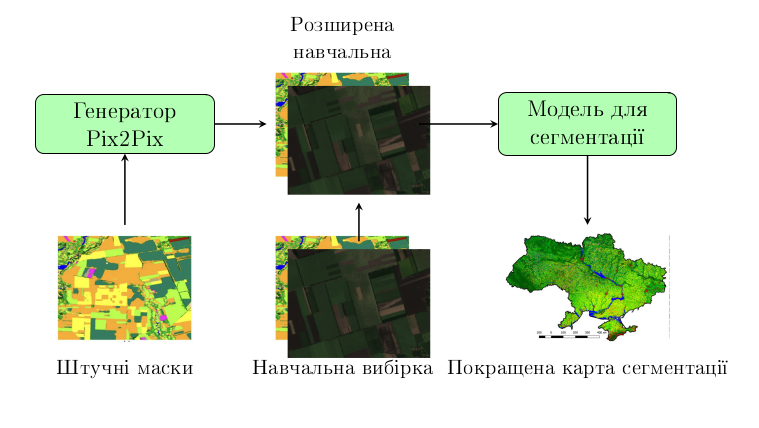
\includegraphics[scale=0.5]{pipline.png}
    \caption{Процес аугментації наборів даних супутникових знімків за допомогою Pix2Pix}
    \label{fig:pipline}
\end{figure}

Наступним важливим питанням є засоби створення штучних масок,
які дозволять збалансувати набір даних. Для вирішення цієї
задачі теж можна використовувати багато підходів, у тому числі і
генеративно-змагальні мережі, проте простішим і, тим не менш,
логічно обґрунтованим є підхід щодо зміни міток класів на вже
існуючих масках, які відповідають справжнім супутниковим знімкам.
Це дозволить бути впевненими у тому, що просторове розташування
класів завжди буде відповідати шаблонам з реального світу.

Для того, щоб змінювати існуючи маски пропонується наступна
стратегія: ми будемо змінювати лише декілька класів на кожній ітерації, що
дозволить наблизити характеристики штучних масок до реальних.
Причому змінювати пропонується класи, які для даного знімку є такими,
що мають найбільшу кількість пікселів. Таким чином можемо
привести алгоритм генерації штучних масок.

\begin{algorithm}[Алгоритм генерації масок] \label{alg:mask_gen} \leavevmode \linebreak
    Параметри: $l$ -- кількість класів, які будуть змінені
    Вхідні дані: навчальна вибірка, бажана кількість пікселів для кожного з класів
    \begin{enumerate}
        \item Визначити які класи не досягли достатньої кількості пікселів та додати їх у чергу
        \item Поки залишились елементи у черзі

              \begin{enumerate}
                  \item Дістати з черги $l$ міток класів $k_1, \dots, k_l$. (Якщо на даній ітерації
                        у черзі менше за $l$, то встановити $l$ таким, що дорівнює
                        довжині черзі).
                  \item Для наступного елемента у наборі даних, отримати маску,
                        в якій усі мітки $l$ класів, які займає найбільше пікселів замінити
                        на $k_1, \dots, k_l$ відповідно
                  \item Зберегти отриману маску
                  \item Додати кількість пікселів за кожним класом згенерованої
                        маски до сумарної кількості пікселів за класами.
                        Якщо для якогось з класів $k_1, \dots, k_l$ ще не досягнута бажана
                        кількість пікселів, то додати такі мітки послідовно у чергу.
              \end{enumerate}
    \end{enumerate}
\end{algorithm}

Як можна побачити даний алгоритм приймає бажану кількість класів,
а не завжди робить розподіл класів наближеним до рівномірного.
Це пов'язано з тим,  що, по-перше, нас може цікавити підвищення якості
семантичної сегментації не усіх класів, а лише певних.
По-друге, намагання отримати рівномірний розподіл може призвести до того,
що частка згенерованих прикладів буде значно переважати частку
справжніх, що може дуже негативно впливати на результати, бо
недоліки, у штучно згенерованих за допомогою генеративно-змагальних
мереж зображень, все ж таки присутні.

\chapconclude{\ref{chap:gans}}

У другому розділі ми зосередились на огляді
генеративних моделей та можливостей їх
застосування для аугментації навчальних вибірок
супутникових знімків.

Перш за все було розглянуто постановку задачі
генерування зображень у математичній постановці та
різні класи генеративних моделей. Ґрунтуючись на недоліках і
перевагах кожного з цих класів, було визначено,
що найбільшу перспективу для вирішення задачі генерації
супутникових зображень мають генеративно-змагальні мережі.

Тож було докладно проаналізовано властивості збіжності цих мереж,
наведено алгоритм навчання та описано основні проблеми, які
виникають з GAN та шляхи їх вирішення.

Через те, що задача аугментації вибірок у нашій постановці вимагає
контролю за міткою класу кожного з пікселів згенерованого зображення,
ми звернулись до генеративно-змагальних мереж, які дозволяють
розв'язувати задачу image-to-image translation. Визначними нейромережевими
архітектурами у цій галузі є Pix2Pix та нащадки, тож було
детально проаналізовано їх застосування до
генерації супутникових знімків.

На сам кінець, був запропонований процес аугментації навчальних вибірок супутникових
знімків, який полягає у тому, що ми, за описаним алгоритмом, спершу
генеруємо маски, які будуть коригувати незбалансованість класів,
а після цього, ґрунтуючись на даних масках, генерувати штучні
супутникові знімки за допомогою
архітектури Pix2Pix та її варіацій.